%%
%% /docs/report/content/chapters/implementation.tex
%%
%% Created by Paul Warkentin <paul@warkentin.email> on 21/07/2018.
%% Updated by Paul Warkentin <paul@warkentin.email> on 26/07/2018.
%%

\section{Implementation}
\label{section:implementation}

We will discuss two different sizes of SSD networks in this project. The SSD 300 and SSD 512 networks accept image inputs of size $300 \times 300$ and $512 \times 512$ respectively. The smaller SSD 300 network is not as precise as the bigger SSD 512 network but can therefore score with a better inference time. \\

Some of the tricks in this implementation will be based on the original Caffe implementation \cite{ssdcfgit}. All presented methods are implemented in Python 3.6\footnote{\url{https://www.python.org/}} making prevalent use of TensorFlow 1.9\footnote{\url{https://www.tensorflow.org/}} and NumPy 1.14\footnote{\url{https://www.numpy.org/}}. The source code is publicly available at \url{https://github.com/paulwarkentin/tf-ssd-vgg}. The \texttt{README.md} provides additional information on how to get started.

\subsection{Model structure}

The model of the SSD network consists of three parts. \\

First, the input image is fed into a classifier network, here called the base network. In this project we use the VGG 16 network for this purpose. The fully connected layers in the standard architecture are replaced by convolutional feature layers.

Secondly, the output of the modified base network is fed into a series of extra feature layers. These layers decrease in size and allow the prediction of detections at multiple scales.

Finally, the output of the extra feature layers plus a selected layer from the base network are used as detection predictors. Each of these layers can produce a fixed set of predictions using a new set of convolutional layers.

\begin{center}
  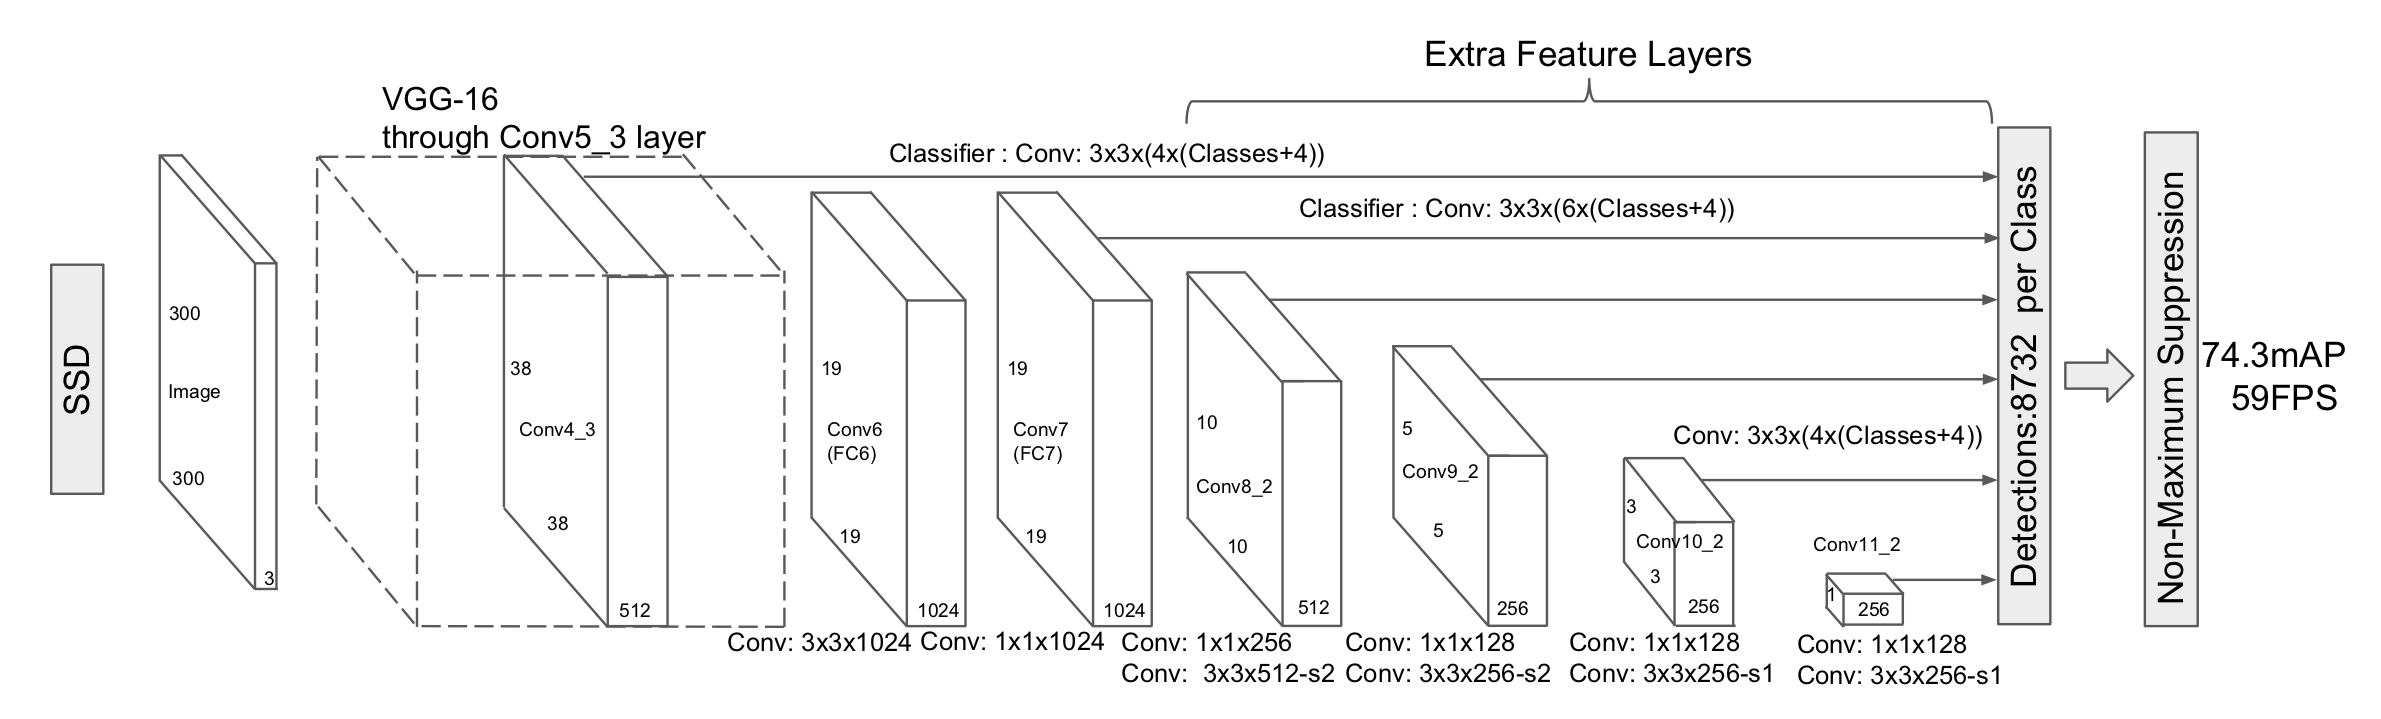
\includegraphics[width=1.0\linewidth]{ssd_architecture.png}
  \captionof{figure}{Architecture of the SSD 300 network.}
\end{center}

The structure above is about the SSD 300 network. The slightly bigger SSD 512 network has two more extra feature layers.

\subsection{MultiBox priors}

MultiBox starts with a fixed set of default anchor boxes as priors for the predictions and attempt to approach the groundtruth bounding boxes using the priors. \\

For each feature layer, we compute default anchor boxes for a given set of aspect ratios and scales. The number of anchor boxes for a feature layer of size $(h, w)$ of $b$ different scales and ratios can be calculated by $b \cdot h \cdot w$. In the implementation of this project we use the following presets for the SSD 300 network.

\begin{center}
  \begin{tabular}{l|c|c|c}
    \textbf{Layer} & \textbf{Height} & \textbf{Width} & \textbf{\# Ratios} \\ \hline
    \texttt{conv4\_3} & 38 & 38 & 4 \\
    \texttt{conv7} & 19 & 19 & 6 \\
    \texttt{conv8\_2} & 10 & 10 & 6 \\
    \texttt{conv9\_2} & 5 & 5 & 6 \\
    \texttt{conv10\_2} & 3 & 3 & 4 \\
    \texttt{conv11\_2} & 1 & 1 & 4
  \end{tabular}
  \captionof{table}{Presets for the SSD 300 network.}
\end{center}

This sums up to a total of 8732 default anchor boxes. The SSD 512 network is defined by the following presets.

\begin{center}
  \begin{tabular}{l|c|c|c}
    \textbf{Layer} & \textbf{Height} & \textbf{Width} & \textbf{\# Ratios} \\ \hline
    \texttt{conv4\_3} & 64 & 64 & 4 \\
    \texttt{conv7} & 32 & 32 & 6 \\
    \texttt{conv8\_2} & 16 & 16 & 6 \\
    \texttt{conv9\_2} & 8 & 8 & 6 \\
    \texttt{conv10\_2} & 4 & 4 & 6 \\
    \texttt{conv11\_2} & 2 & 2 & 4 \\
    \texttt{conv12\_2} & 1 & 1 & 4
  \end{tabular}
  \captionof{table}{Presets for the SSD 300 network.}
\end{center}

This sums up to a total of 24564 default anchor boxes.

\subsection{Matching strategy}

Before the training step, we need to match the groundtruth boxes to the previous calculated default anchor boxes. The image below describes the logic of this step well. The bounding box of the dog is matched to the red dotted anchor box in the $4 \times 4$ feature layer but not to any shown box in the $8 \times 8$ feature layer. The criteria of a match is given by the Intersection of Union (in short: IoU) and a given threshold, here $\frac{1}{2}$. The IoU is dependent on the location, size and aspect ratios of the boxes. The bounding box of the cat on the other hand is matched to the blue dotted anchor box on the $8 \times 8$ feature layer.

\begin{center}
  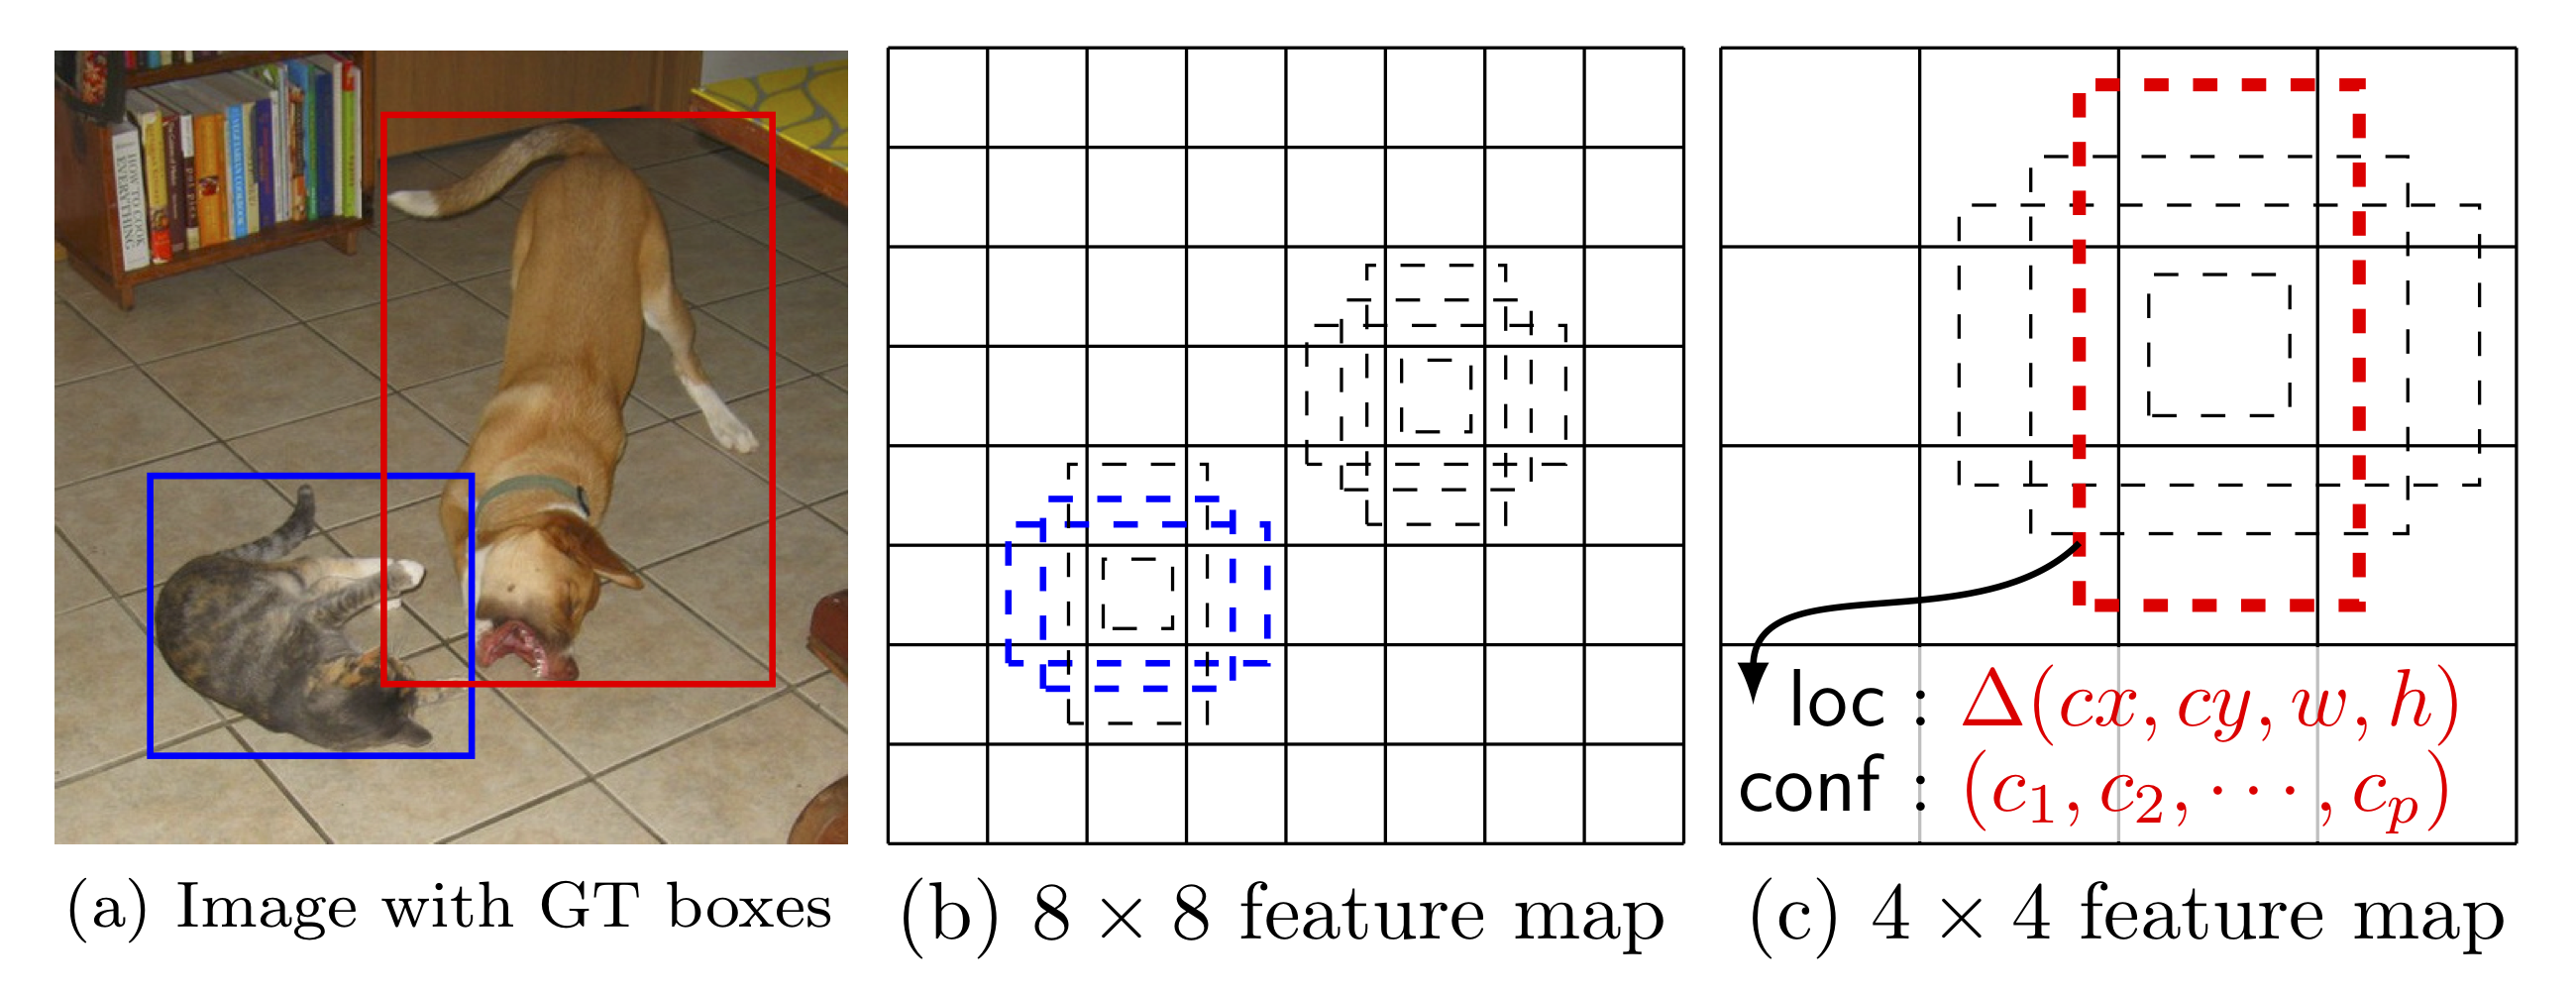
\includegraphics[width=0.8\linewidth]{default_anchor_boxes.png}
  \captionof{figure}{Matching default anchor boxes.}
\end{center}

In this project, we follow a certain strategy for finding those matches. First, we match each groundtruth box to the default anchor box with the highest IoU. Then, each other default anchor box is matched to any groundtruth box with an IoU over a given threshold, here $\frac{1}{2}$.

\subsection{Training objective}

The loss function is the sum of two components.

\begin{itemize}
  \item \textbf{Confidence loss:} this loss measures the confidence of the predicted class of the computed bounding box. To compute this loss, categorical softmax cross-entropy is used.
  \item \textbf{Localization loss:} this loss measures the distance of the computed bounding box from the groundtruth box. To compute this loss, the L2-Norm is used.
\end{itemize}

Let $x_{ij}^p \in \{0, 1\}$ be the status of matching the $i$-th default anchor box to the $j$-th groundtruth box of class $p$. The set $X_P$ contains all default anchor boxes that were matched to a groundtruth box, the set $X_N$ on the other hand contains all unmatched anchor boxes. \\

The confidence loss is calculated for positive and negative samples by
\begin{equation*}
  L_{conf}(x, c) = - \sum_{i \in X_P} x_{ij}^p \log(\hat{c}_i^p) - \sum_{i \in X_N} \log(\hat{c}_i^0),
\end{equation*}
where $\hat{c}_i^p$ is the softmax function over confidences $c_i^p$ of class $p$,
\begin{equation*}
  \hat{c}_i^p = \frac{\exp(c_i^p)}{\sum_p \exp(c_i^p)}.
\end{equation*}
After the matching step, most of the default anchor boxes are not matched with any object, i.e. they are negatives. To compensate this imbalance of positive and negative samples, we perform hard negative mining. We sort the confidence losses of the negative samples in descending order and take only the samples with the highest loss so that the ratio of positive to negative samples is 1:3. \\

The localization loss is calculated for positive samples by using the predicted box $b$ and the groundtruth box $g$,
\begin{equation*}
  L_{loc}(x, b, g) = \sum_{i \in X_P} \sum_m x_{ij}^p \text{smooth}_{L1}(b_i^m - \hat{g}_j^m),
\end{equation*}
where $m \in \{cx, cy, w, h\}$ and $\hat{g}_j$ is the SSD encoding of the $j$-th groundtruth box using the $i$-th default anchor box $d_i$ defined by
\begin{alignat*}{2}
  & \hat{g}_j^{cx} = \frac{1}{d_i^w} (g_j^{cx} - d_i^{cx}),\ \ \ && \hat{g}_j^{cy} = \frac{1}{d_i^h} (g_j^{cy} - d_i^{cy}), \\
  & \hat{g}_j^{w} = \log\Big(\frac{g_j^w}{d_i^w}\Big), && \hat{g}_j^{h} = \log\Big(\frac{g_j^h}{d_i^h}\Big).
\end{alignat*}
The smooth L1-Norm is defined as
\begin{equation*}
  \text{smooth}_{L1}(y) = \begin{cases}
    \frac{1}{2} y^2 & \text{if} \ \lvert y \rvert \leq 1 \\
    \lvert y \rvert - \frac{1}{2} & \text{otherwise}.
  \end{cases}
\end{equation*}

The overall training objective is then calculated by adding and normalizing the latter two losses,
\begin{equation*}
  L(x, c, b, g) = \frac{1}{N} (L_{conf}(x, c) + L_{loc}(x, b, g)).
\end{equation*}
If the number of positive samples $N$ is equal to zero, we set the loss to zero.

\subsection{Data augmentation}

Before training, various data augmentation tricks are randomly applied to the input images to increase the number of samples and to reduce overfitting of the network. \\

First, the colors of the image are randomly distorted choosing one of four distortion packages. Each package adjusts the brightness, saturation, hue and contrast of the image with random parameters. Each package applies the distortions in a different order. After the color distortions, the RGB channels of the image are randomly reordered. \\

Secondly, the image is expanded, i.e. the image is randomly placed on a canvas up to four times bigger than the image itself. The background color of the canvas is set to the mean value of the dataset that was used to train the base network. All bounding boxes are transformed accordingly. \\

Thirdly, the image is randomly cropped so that the cropped image contains at least $\frac{1}{2}$ of any bounding box. All bounding boxes are transformed accordingly. \\

Lastly, the image is randomly flipped horizontally.

\subsection{Evaluation metric}

To evaluate the training results the mean average precision (in short: mAP) is used. mAP is often used in object detection. The metric is calculated using the precision and the recall of objects of one class.
\begin{itemize}
  \item \textbf{Precision:} measures how accurate the prediction is, i.e. the percentage of the positive predictions that are correct,
  \begin{equation*}
    \text{Precision} = \frac{TP}{TP + FP}.
  \end{equation*}
  \item \textbf{Recall:} measures how good all the positives were found,
  \begin{equation*}
    \text{Recall} = \frac{TP}{TP + FN}.
  \end{equation*}
\end{itemize}

The average precision is then calculated by computing the area under thre precision-recall curve. This value is computed for every class. The mAP is then the mean of the average precision values of all classes.
